%!TEX root=paper.tex
\section{Evaluation}
\label{sec:evaluation}

In this chapter, we will investigate the scalability of Gilbert and its performance compared to famous hand-tuned ML algorithms.
We show that Gilbert is not only easily usable in terms of programming but also produces results with decent performance.

\textbf{Experimental Setup}. For our evaluation, we use a $25$ machine cluster with 32 gigabytes of main memory per computer.
Each machine is equipped with $2$ AMD Opterons 6128 CPUs, each of them having $8$ cores.
The CPUs run at a speed of 2 gigahertz. We employ Apache Spark-2.0.0~\cite{spark} for our test runs with the Spark execution engine.
For the Flink execution engine, we use Apache Flink-1.1.3~\cite{flink}. As the underlying distributed file system both systems use Apache Hadoop-2.7.3~\cite{hadoop:2008a}. All experiments have been executed five times and the mean of the measurement is reported.

\subsection{Scalability}

The scalability evaluation investigates how Gilbert behaves under increasing work loads and how well it can exploit varying cluster sizes.
As we have implemented Gilbert to provide a scalable linear algebra environment, it is important that it can process data sizes exceeding the main memory of a single machine.

%\subsubsection{Matrix Multiplication}
%\label{subsec:mm}

\textbf{Matrix Multiplication}. As a first benchmark, we choose the matrix multiplication $A\times B$ with $A,B \in \mathbb{R}^{n\times n}$ with $n$ being the dimensionality. The matrix multiplication operation is demanding, both in CPU load as well as network I/O as it requires two network shuffles. The matrices $A$ and $B$ are sparse matrices with uniformly distributed non-zero cells. They are randomly generated prior to the matrix multiplication with a sparsity of $0.001$. As a baseline, we run the same matrix multiplication on a single machine of the cluster using Gilbert's local execution engine. The Flink and Spark execution engines are both started with 20 gigabytes of main memory for their task managers and they distribute the work equally among all worker nodes. In the first experiment, we fixed the block sizes to $500 \times 500$ and set the number of cores to $50$. We then increased the dimensionality $n$ of $A$ and $B$ to observe the runtime behavior. The resulting execution times for the local, Flink and Spark execution engines are shown in \cref{fig:mmLoadRuntime}. In the second experiment, we investigate the scaling behavior of Gilbert with respect to the cluster size. In order to observe the inflicted communication costs, we keep the work load per core constant while increasing the number of cores. For this experiment we vary the number of cores from $1$ to $100$ and scale $n$ such that $n^3/\#cores$ is constant. We started with $n=7500$ for a single core and reached $n=35000$ on $100$ cores. The results of the experiment are shown in \cref{fig:mmNodesRuntime}. On a single machine, we are able to execute the matrix multiplication for dimensionalities up to $n=10000$ before the system ran out of memory. We can see that the local execution performs better for dimensionalities $n \le 5000$. That is expected since the matrix still fits completely in the main memory of a single machine and the distributed execution adds some significant communication overhead and job start up latency. For matrices with $n>5000$, Spark starts to calculate the matrix multiplication faster than the local executor. The Flink execution engine does not beat the local computation for sizes which are manageable by a single machine, though. We also see that Gilbert can handle matrix sizes which scale far beyond the memory capacity of a single machine. The results depicted in \cref{fig:mmNodesRuntime} indicate for both execution engines decent scale-out behavior. Especially for the number of cores $\le 15$, we observe for Flink and Spark an almost horizontal line. From this point onwards, the scaling of Flink degrades faster than Spark's scaling. The Spark execution engine requires 90 seconds to calculate the matrix multiplication with $n=35000$ on $100$ cores. That is only a slowdown by a factor of $1.5$, if compared to the matrix multiplication with $n=7500$ on a single core, which takes 65 seconds to finish.

\begin{figure}[!h]
	\centering
	\begin{subfigure}{\dualpgfwidth}
		\begin{tikzpicture}
			\begin{loglogaxis}[
				xlabel={Dimensionality $n$},
				ylabel={Execution time $t$ in s},
				width=\dualpgfwidth,
				legend entries={Local, Spark, Flink},
				legend pos=north west,
			]
			\addplot[
				color=blue,
				mark=x,
			] table[
				x=RowsA,
				y=Time,
			]
			{data/matrixMultLoad/matrixMultLoadReference};
			\addplot[
				color=red,
				mark=o,
			] table[
				x=RowsA,
				y=Time,
			]
			{data/matrixMultLoad/matrixMultLoadSpark};
			\addplot[
				color=teal,
				mark=triangle,
			] table[
				x=RowsA,
				y=Time,
			]
			{data/matrixMultLoad/matrixMultLoadStratosphere};
			\end{loglogaxis}
		\end{tikzpicture}
		\caption{}
		\label{fig:mmLoadRuntime}
	\end{subfigure}
	\begin{subfigure}{\dualpgfwidth}
		\begin{tikzpicture}
			\begin{semilogxaxis}[
				xlabel={Number of cores},
				ylabel={Execution time $t$ in s},
				legend pos=north west,
				legend entries={Spark, Flink},
				ymin=0.0,
				ymax=275,
				width=\dualpgfwidth,
			]
			\addplot[
				color=red,
				mark=o,
			] table[
				x=Parallelism,
				y=Time,
			]
			{data/matrixMultCores/matrixMultCoresSpark};
			\addplot[
				color=teal,
				mark=triangle,
			] table[
				x=Parallelism,
				y=Time,
			]
			{data/matrixMultCores/matrixMultCoresStratosphere};
			\end{semilogxaxis}
		\end{tikzpicture}
		\caption{}
		\label{fig:mmNodesRuntime}
	\end{subfigure}
	\caption{Scalability of matrix multiplication. \subref{fig:mmLoadRuntime} Execution time of matrix multiplication depending on the data size. \subref{fig:mmNodesRuntime} Execution time of matrix multiplication depending on the cluster size with constant work load per core.}
	\label{fig:mmScalability}
\end{figure}

%\subsubsection{Gaussian Non-negative Matrix Factorization}
%\label{subsec:NMF}

\textbf{Gaussian Non-negative Matrix Factorization}. As second benchmark for evaluating the scalability properties, we choose the Gaussian non-negative matrix factorization (GNMF) algorithm~\cite{seung:anips2001a}.
GNMF finds for a given matrix $V \in \mathbb{R}^{d\times w}$ a factorization $W \in \mathbb{R}^{d\times t}$ and $H \in \mathbb{R}^{t\times w}$ such that $V\approx W H$ holds.
For our evaluation, we calculate one step of the GNMF algorithm.
We set $t=10$, $w=100000$ and vary the number of rows $d$ of $V$.
The matrix $V\in\mathbb{R}^{d\times 100000}$ is a sparse matrix whose sparsity is set to $0.001$.
The non-zero cells of $V$ are uniformly distributed.
As a baseline, we run the GNMF on a single machine of the cluster using the local execution engine.
Like for the matrix multiplication benchmark, the task manager of Spark and Flink are started with 20 gigabytes of memory and both systems use the same scheduling strategy keeping the work load on all nodes equally distributed.
In the first experiment we fix the number of cores to $50$.
We start with $d=500$ and increase the number of rows of $V$ to $150000$.
The block size of Gilbert is set to $500 \times 500$.
In order to compare the results with the optimized NMF MapReduce implementation proposed in~\cite{liu:2010a}, we re-implemented the algorithm using the Spark and Flink runtime system.
This hand-tuned implementation, henceforth denoted as HT-GNMF (HT in the graphs), is also executed on $50$ cores.
The execution times of HT-GNMF and Gilbert's GNMF are shown in \cref{fig:nmfLoadRuntime}.
In the second experiment of the GNMF benchmark, we analyze how Gilbert scales-out when increasing the cluster size while keeping the work load for each core constant.
We vary the cluster size from $1$ core to $100$ cores and scale the number of documents $d$ accordingly.
Initially we start with $1000$ documents and, consequently, calculate the matrix factorization for $100000$ documents on $100$ cores.
The results of this experiment are shown in \cref{fig:nmfNodesRuntime}.

\begin{figure}[!h]
	\centering
	\begin{subfigure}{\dualpgfwidth}
		\begin{tikzpicture}
			\begin{loglogaxis}[
				xlabel={Rows $d$ of $V$},
				ylabel={Execution time $t$ in s},
				width=\dualpgfwidth,
				legend pos=north west,
				legend columns=2,
				legend entries={Local, Spark, Flink, HT Spark, HT Flink},
				ymax=8000,
			]
			\addplot[
				color=blue,
				mark=x,
			] table[
				x=Rows,
				y=Time,
			]
			{data/nnmfStepLoad/nnmfStepLoadReference};
			
			\addplot[
				color=red,
				mark=o,
			] table[
				x=Rows,
				y=Time,
			]
			{data/nnmfStepLoad/nnmfStepLoadSpark};
			
			\addplot[
				color=teal,
				mark=triangle,
			]table[
				x=Rows,
				y=Time,
			]
			{data/nnmfStepLoad/nnmfStepLoadStratosphere};
			\addplot[
				color=black,
				mark=diamond,
			]table[
				x=rowsV,
				y=time,
			]
			{data/nnmfStepLoad/gnmfStepLoadSpark};
			\addplot[
				color=magenta,
				mark=square,
			]table[
				x=rowsV,
				y=time,
			]
			{data/nnmfStepLoad/gnmfLoadStratosphere};
			\end{loglogaxis}
		\end{tikzpicture}
		\caption{}
		\label{fig:nmfLoadRuntime}
	\end{subfigure}
	\begin{subfigure}{\dualpgfwidth}
		\begin{tikzpicture}
			\begin{semilogxaxis}[
				xlabel={Rows $d$ of $V$},
				ylabel={Speedup of HT-GNMF on Spark},
				width=\dualpgfwidth,
				ymin=0,
				legend entries={Spark,Flink},
				legend pos=north west,
			]
			\addplot[
				color=red,
				mark=o,
			] table[
				x=Rows,
				y=Speedup,
			]
			{data/nnmfStepLoad/gnmfStepLoadSpeedupSpark};

			\addplot[
				color=teal,
				mark=diamond,
			] table[
				x=Rows,
				y=Speedup,
			]
			{data/nnmfStepLoad/gnmfStepLoadSpeedupStratosphere};
			\end{semilogxaxis}
		\end{tikzpicture}
		\caption{}
		\label{fig:gnmfSpeedup}
	\end{subfigure}
	\begin{subfigure}{\dualpgfwidth}
		\begin{tikzpicture}
			\begin{semilogxaxis}[
				xlabel={Number of cores},
				ylabel={Execution time $t$ in s},
				ymin=0,
				legend entries={Spark, Flink},
				legend pos=north west,
				width=\dualpgfwidth,
			]
			\addplot[
				color=red,
				mark=o,
			] table[
				x=Parallelism,
				y=Time,
			]
			{data/nnmfStepCores/nnmfStepCoresSpark};

			\addplot[
				color=teal,
				mark=diamond,
			] table[
				x=Parallelism,
				y=Time,
			]
			{data/nnmfStepCores/nnmfStepCoresStratosphere};
			\end{semilogxaxis}
		\end{tikzpicture}
		\caption{}
		\label{fig:nmfNodesRuntime}
	\end{subfigure}
	\caption{Scalability of GNMF on a $50$-core cluster. \subref{fig:nmfLoadRuntime} Execution time of one GNMF step depending on the data size. \subref{fig:gnmfSpeedup} Speedup of HT-GNMF running on Spark compared to Gilbert's GNMF using the Spark and Flink execution engine, respectively. \subref{fig:nmfNodesRuntime} Execution time of one GNMF step depending on the cluster size with constant work load per core.}
	\label{fig:nmfBenchmark}
\end{figure}

The local executor can be applied to sizes of $d$ ranging from $500$ to $1500$ rows, before the data exceeded the available main memory of a single computer.
As expected, the local execution performs far better for these data sizes than the distributed execution with Flink.
However, the GNMF and the HT-GNMF executed on Spark outperformed the local execution.
The distributed systems can also be used for data sizes which exceed the memory of a single computer.
Both distributed execution engines scale well up to the point where Spark and Flink can no longer keep the data in memory and have to spill it.
The runtime of HT-GNMF running on Spark, the Flink and the Spark executor differ for varying data sizes almost by a constant factor.
The fastest implementation for $d\le 100000$ is the HT-GNMF algorithm running on Spark.
The speedup of HT-GNMF running on Spark compared to GNMF on Spark's and Flink's executor is shown in \cref{fig:gnmfSpeedup}.
It can be seen that HT-GNMF runs approximately $1.7$ times faster than Gilbert's GNMF using the Spark executor.
Compared to the Flink execution engine, we can observe that HT-GNMF runs faster and faster for increasing $d$.
HT-GNMF achieves a speedup of approximately $16$ for $d=50000$.
The runtime behavior of HT-GNMF running on Flink is interesting.
At first, it performs rather poorly compared to its Spark counterpart.
However, for $d>100000$ it suddenly outperforms the Spark implementation.
Thus, GNMF scales better if it is executed on Flink. 
Even though, Gilbert can not even reach the performance of HT-GNMF, the development using Gilbert was considerably easier.
One GNMF step can be programmed in five lines of Gilbert code, whereas we needed $28$ lines of Scala code for Spark's HT-GNMF and $70$ lines of Scala code for Flink's HT-GNMF.
Not only did we have to know how to program Spark and Flink, but it also took us quite some time to verify the correct functioning of both implementations.
The verification was made significantly more difficult and time-consuming due to a programming bug we introduced.
The debugging process showed us quite plainly how tedious the development process even with systems like Spark and Flink can be.
Thus, the productivity increase gained by using a high-level declarative programming language for linear algebra must not be neglected and compensates for the performance loss.
\cite{alvaro:2010a} made a similar observations while developing a declarative programming language for distributed systems programming.
The scale-out behavior of the Flink and Spark execution engines \cref{fig:nmfNodesRuntime} both show good results for $\#cores \le 5$.
For higher degrees of parallelism, Flink's performance quickly deteriorates.
On $50$ cores, Flink needs 1082 seconds, whereas Spark needs only 113 seconds.
That vast performance decline is most likely caused by data spilling at some internal operation.
The runtime on Spark with $100$ cores is only two times slower than the runtime on a single core with the same work load per core.

% \subsection{Optimizations}

% In this section, we want to evaluate the effects Gilbert's optimizer has on the runtime of programs.
% For this purpose, we execute one GNMF step on Gilbert's Stratosphere and Spark execution engine using the same settings as in \cref{subsec:NMF}.
% However, this time we disable the transpose pushdown and matrix-multiplication reordering optimization.
% The results are shown in \cref{fig:nnmfLoadOptimization}.

% \begin{figure}
% 	\centering
% 	\begin{subfigure}[t]{\dualpgfwidth}
% 		\begin{tikzpicture}
% 			\begin{semilogxaxis}[
% 				xlabel={Rows $d$ of $V$},
% 				ylabel={Execution time $t$ in s},
% 				legend pos=north west,
% 				legend entries={Optimized Spark, Optimized Stratosphere, Non-optimized Spark, Non-optimized Stratosphere},
% 				width=\dualpgfwidth,
% 			]
			
% 			\addplot[
% 				color=red,
% 				mark=o,
% 			] table[
% 				x=Rows,
% 				y=Time,
% 			]
% 			{data/nnmfStepLoadNoOp/nnmfStepLoadSpark};
			
% 			\addplot[
% 				color=teal,
% 				mark=triangle,
% 			]table[
% 				x=Rows,
% 				y=Time,
% 			]
% 			{data/nnmfStepLoadNoOp/nnmfStepLoadStratosphere};

% 			\addplot[
% 				color=blue,
% 				mark=x,
% 			] table[
% 				x=Rows,
% 				y=Time,
% 			]
% 			{data/nnmfStepLoadNoOp/nnmfStepNoOpLoadSpark};

% 			\addplot[
% 				color=black,
% 				mark=diamond,
% 			]table[
% 				x=Rows,
% 				y=Time,
% 			]
% 			{data/nnmfStepLoadNoOp/nnmfStepNoOpLoadStratosphere};
			
% 			\end{semilogxaxis}
% 		\end{tikzpicture}
% 		\caption{}
% 		\label{fig:nnmfLoadOptimization}	
% 	\end{subfigure}
% 	\begin{subfigure}[t]{\dualpgfwidth}
% 		\begin{tikzpicture}
% 			\begin{semilogxaxis}[
% 				xlabel={Rows $d$ of $V$},
% 				ylabel={Speedup},
% 				legend pos=north west,
% 				legend entries={Optimized Spark, Optimized Stratosphere},
% 				width=\dualpgfwidth,
% 			]
			
% 			\addplot[
% 				color=red,
% 				mark=o,
% 			] table[
% 				x=Rows,
% 				y=Speedup,
% 			]
% 			{data/nnmfStepLoadNoOp/gnmfStepLoadSpeedupSpark};
			
% 			\addplot[
% 				color=teal,
% 				mark=triangle,
% 			]table[
% 				x=Rows,
% 				y=Speedup,
% 			]
% 			{data/nnmfStepLoadNoOp/gnmfStepLoadSpeedupStratosphere};			
% 			\end{semilogxaxis}
% 		\end{tikzpicture}
% 		\caption{}
% 		\label{fig:gnmfLoadOptimizationSpeedup}
% 	\end{subfigure}
% 	\caption{Effect of Gilbert's optimizations using the example of a single GNMF step executed on a $50$-core cluster. \subref{fig:nnmfLoadOptimization} Execution time of the optimized and non-optimized GNMF step depending on the input size. \subref{fig:gnmfLoadOptimizationSpeedup} Speedup of the optimized GNMF step with respect to the non-optimized GNMF step depending on the input size.}
% \end{figure}

% We can observe that the Gilbert optimizer has a significant effect on the runtime of GNMF.
% The optimized Gilbert program runs on both distributed engines faster than it's non-optimized counterparts.
% Interestingly, the Spark execution engine seems to benefit more from the optimizer than the Stratosphere executor.
% The speedups of the optimized GNMF step with respect to its non-optimized counterparts are shown in \cref{fig:gnmfLoadOptimizationSpeedup}
% For the optimized program running on Spark's execution engine, a steadily ascending speedup, except for $d=500$, can be observed.
% The optimized Spark version runs about $18$ times faster than the non-optimized program for $d=10000$.
% In contrast to that, Stratosphere shows a constant speedup of roughly $1.7$ between the optimized and non-optimized version.

% It is not yet known what causes these different speedups.
% However, looking at the GNMF formula in \cref{lst:nmf}, it becomes obvious why the optimization works.
% There are two matrix multiplications that can be optimized: $W^T WH$ in line $6$ and $WHH^T$ in line $7$.
% Keeping in mind that $W\in \mathbb{R}^{d\times 10}$ and $H\in \mathbb{R}^{10 \times 100000}$, we can assess the different strategies.
% The non-optimized version would execute the matrix multiplications due to left-associativity from left to right:

% \begin{displaymath}
% 	\overbrace{\underbrace{\left(W^T W\right)}_{\in \mathbb{R}^{10\times 10}}H}^{\in\mathbb{R}^{10\times 100000}}
% \end{displaymath}

% and

% \begin{displaymath}
% 	\overbrace{\underbrace{\left(WH\right)}_{\in \mathbb{R}^{d \times 100000}}H^T}^{\in \mathbb{R}^{d\times 10}}
% \end{displaymath}

% For the first matrix multiplication, the execution order is optimal, since the intermediate result of $W^T W$ is much smaller than $WH$.
% However, for the second matrix multiplication, the execution order is far from optimal.
% The left-associativity produces an intermediate matrix result of size $d\times 100000$.
% For large $d$ this matrix becomes really huge.
% Additionally, the intermediate result is dense, because the operands $W$ and $H$ are dense, as well.
% By changing the execution order, we can decrease the size of the intermediate result significantly.

% \begin{displaymath}
% 	\overbrace{W\underbrace{\left(HH^T\right)}_{\in \mathbb{R}^{10 \times 10}}}^{\in \mathbb{R}^{d\times 10}}
% \end{displaymath}

% The Gilbert optimizer first detects the matrix multiplication reordering and then changes it so that the maximum intermediate result is minimized.
% That is the reason why the optimized GNMF program runs clearly faster.

\subsection{PageRank}

In this section, we want to investigate how well the PageRank algorithm~\cite{page:1999a} implemented in Gilbert performs compared to a specialized implementation.
We expect that the Gilbert runtime adds some overhead.
Furthermore, the high-level linear algebra abstraction of Gilbert might make it difficult to exploit certain properties to speed up the processing.
We first execute PageRank directly in Gilbert, given the Gilbert code \cref{lst:gilbertPageRank}, and then run them directly on Flink and Spark.
In contrast to Gilbert, the direct implementation requires a deep understanding of the underlying runtime system.
Furthermore, the distributed implementation is far from trivial compared to the linear algebra representation of the original problem.

\begin{listing}[!h]
	\begin{CenteredBox}
		\begin{lstlisting}[language=Matlab,
		commentstyle=\color{black},
		  stringstyle=\color{black},
		  keywordstyle=\color{black}\bfseries,
		  morekeywords={ones, fixpoint},]
% load adjacency matrix
A = load();
maxIterations = 10;
d = sum(A, 2); % outdegree per vertex
% create the column-stochastic transition matrix
T = (diag(1 ./ d) * A)'; 
r_0 = ones(numVertices, 1) / numVertices; % initialize the ranks
e = ones(numVertices, 1) / numVertices;
% PageRank calculation
fixpoint(r_0, @(r) .85 * T * r + .15 * e, maxIterations)
		\end{lstlisting}
	\end{CenteredBox}
	\caption{Gilbert PageRank implementation.}
	\label{lst:gilbertPageRank}
\end{listing}

The Spark and Flink implementation of PageRank works as follows.
The PageRank vector is represented by a set of tuples $(w_i, r_i)$ with $w_i$ denoting the web site $i$ and $r_i$ being its rank.
The adjacency matrix is stored row-wise as a set of tuples $(w_i, A_i)$ with $w_i$ denoting the web site $i$ and $A_i$ being its adjacency list.
For the adjacency list $A_i$, it holds that $w_j \in A_i$ if and only if there exists a link from web site $i$ to $j$.
The next PageRank vector is calculated as follows.
The PageRank $r_i$ of web site $i$ is joined with its adjacency list $A_i$.
For each outgoing link $w_j \in A_i$ a new tuple $(w_j, 0.85r_i/\left|A_i\right|)$ with the rank of $i$ being divided by the number of outgoing links is created.
In order to incorporate the random jump behavior to any available web site, a tuple $(w_i, 0.15/|w|)$, with $|w|$ being the number of all web sites, is generated for each web site $i$.
In order to compute the next PageRank vector, all newly generated tuples are grouped according to their ID.
The resulting groups are reduced by adding up all partial rank values giving the new PageRank vector.
These steps constitute a single PageRank iteration whose data flow plan is depicted in \cref{fig:pageRankDataFlow}.

\begin{figure}[!h]
	\centering
	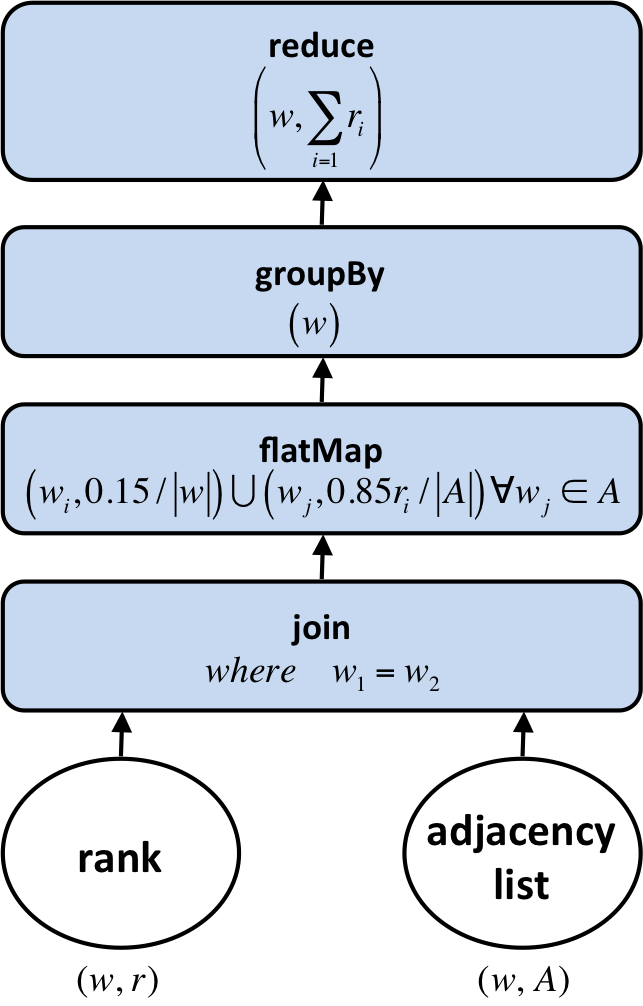
\includegraphics[width=.3\linewidth]{images/pageRankStep.png}
	\caption{Data flow of one iteration of the PageRank algorithm for Spark and Flink.}
	\label{fig:pageRankDataFlow}
\end{figure}

\textbf{Experiment}. For comparison, $10$ steps of the PageRank algorithm for varying sizes of the adjacency matrix $A$ are calculated.
The randomly generated adjacency matrix $A$ is a sparse matrix of size $n \times n$ with a sparsity of $0.001$.
The computation is executed on $50$ cores with a block size of $500 \times 500$.
The execution times are depicted in \cref{fig:pageRankResults}.

\begin{figure}[t!]
	\centering
	\begin{subfigure}[h]{\dualpgfwidth}
		\begin{tikzpicture}
			\begin{loglogaxis}[
				xlabel={Number of vertices $n$},
				ylabel={Execution time $t$ in s},
				legend pos=north west,
				legend entries={Gilbert Spark, Gilbert Flink, Specialized Flink, Specialized Spark},
				width=\dualpgfwidth,
			]
			
			\addplot[blue,
				mark=x,
			] table[
				x=NumVertices,
				y=Time,
			]
			{data/pagerank/pagerankSpark};

			\addplot[red,
				mark=o,
			] table[
				x=NumVertices,
				y=Time,
			]
			{data/pagerank/pagerankStratosphere};

			\addplot[teal,
				mark=diamond,
			] table[
				x=rows,
				y=time,
			]
			{data/pagerank/pagerankBenchStratosphere};

			\addplot[black,
				mark=triangle,
			] table[
				x=rows,
				y=time,
			]
			{data/pagerank/pagerankBenchSpark};
			\end{loglogaxis}
		\end{tikzpicture}
		\caption{}
		\label{fig:pageRankResults}
	\end{subfigure}
	\begin{subfigure}[h]{\dualpgfwidth}
		\begin{tikzpicture}
			\begin{semilogxaxis}[
				xlabel={Number of vertices $n$},
				ylabel={Speedup},
				legend pos=north west,
				legend entries={Specialized Spark, Specialized Flink},
				width=\dualpgfwidth,
			]
			
			\addplot[blue,
				mark=x,
			] table[
				x=NumVertices,
				y=Speedup,
			]
			{data/pagerank/pagerankSpeedupSpark};

			\addplot[red,
				mark=o,
			] table[
				x=NumVertices,
				y=Speedup,
			]
			{data/pagerank/pagerankSpeedupStratosphere};
			\end{semilogxaxis}
		\end{tikzpicture}
		\caption{}
		\label{fig:pageRankSpeedup}
	\end{subfigure}
	\caption{Comparison of Gilbert's PageRank implementation with specialized algorithms on Spark and Flink running on $50$-core cluster. \subref{fig:pageRankResults} Execution time of $10$ steps of the PageRank algorithm depending on the adjacency matrix's size. \subref{fig:pageRankSpeedup} Speedup of specialized algorithms with respect to Gilbert's implementations.}
	\label{fig:pageRankEvaluation}
\end{figure}

The graphs shows that the directly implemented PageRank algorithm runs faster than Gilbert's versions of PageRank \cref{fig:pageRankResults}.
Furhtermore, the specialized algorithms show a better scalability.
The speedup of the specialized algorithms with respect to Gilbert's implementations for this experiment is shown in \cref{fig:pageRankSpeedup}.
For $n\le 25000$, the hand-tuned algorithms running on Spark and Flink show a similarly increasing speedup.
The Flink and Spark version achieve a speedup of approximately $14$ and $10$ for $n=50000$, respectively.
For $n\ge 50000$ Spark seems to exhibit a constant speedup.
The performance difference between the specialized algorithm and Gilbert's version can be explained by considering the different execution plans.
As shown in \cref{fig:pageRankDataFlow}, each iteration of the specialized PageRank algorithm comprises one join, one group reduce and one flat map operation.
In contrast, each iteration of Gilbert's PageRank implementation requires two cross, two join and one reduce operation.
Comparing the specialized algorithm with Gilbert's implementation, it can be clearly seen that the high-level linear algebra representation adds three additional operations, with one of them being highly expensive.
Therefore, it is not surprising that the specialized PageRank algorithm performs better.

